\section{Clouds role in the climate system} \label{sec:cloud_in_climate_system}
%  - clouds, climate and machine learning
Clouds play an important role in the climate system. Both affecting the radiative budget and the hydrological cycle. Understanding how clouds form in the complex system of the atmosphere involves both knowledge about the large scale influence by the circulation and the small scale influenced by aerosols. Clouds are composed of liquid droplets, ice crystal or both. To this day the micro-physics of all phases are not fully understood. Here mixed phase clouds, consisting of both liquid and ice, shows to be the most difficult. 
\\ \\ 
Climate models are the most useful tool for studying the past, present and future climate. Clouds and aerosols are acknowledged as the factors contributing with the largest uncertainty to the \acrfull{ecs}. Also known as global mean temperature increase as a consequence of doubling of the pre-industrial levels of $CO_2$ (280 \acrshort{ppm}). \textbf{kilde AR5} \textit{It remains unclear to which level of sophistication is adequate to model their effect om climate.} \textbf{Siter ch7 AR5}.
\\ \\
%\textbf{Make sure you include everything that's related to parametrised processes.}
It is understood that cloud formation requires suitable aerosols and sufficient supersaturation. \textit{Aerosols} include both gases and solid particles suspended in air. They interact with the clouds by serving as particles which vapour and ice can condensate or deposit upon. The different phases require different properties and the nuclei are called \acrshort{ccn} for liquid droplets and \acrshort{inp} for ice crystals. Saturation is usually achieve by a temperature decrease in rising air masses. %Thus the stability of the atmosphere  plays a key role for convective motions.
%\textbf{Legg inn bilde a skyer en i is fase og en i liquids. Skriv noe som "the sharp outoline suggest that the cloud is consisting of liquid droplets, even at temperagtures below 0."}
%The negative temperature decreases by height is often referred to as the lapse rate, $\Gamma_{s, d}$. 
\\ \\ 
Growth processes are phase dependant. Liquid droplet grows by diffusion and later by collision and coalescence. At temperatures -38 $^oC$ \textbf{kilde Lohmann} they will spontaneously freeze and could play the role as INP. When both phases are present in a cloud, the saturation vapour pressure over ice is higher than over liquid. This may cause the droplets to evaporate and deposit on to the ice crystals. This is called the Wegeron-Bergeron-Findeisen process. Clouds consisting purely of ice crystals first grow by deposition of vapour then by aggregation. 
\\ \\ 
% Lots of different processes occurring simultaneously on different scales 
The complex nature of clouds originates from lots of different processes occurring simultaneously on different scales. Incorporating all these interactions into a model framework has proven to be difficult. \textbf{Finn multiple sources} 
%\textbf{Trude, should I explain convections and fronts? Mention cumulus, cirrus and stratus?}

\section{Clouds in the current climate} \label{sec:intro_cloud_current_climate}
%\begin{figure}[h] % small h, setter den rett under teksten.
%    \centering
%    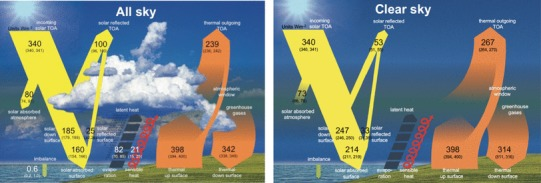
\includegraphics[scale = 7]{Chapter1_Intro/images/both_wild2019.jpg}
%    \caption{The all-sky and the clear sky. Figure 14 Wild 2019. Ikke i bruk vennligst kommenter om denne er bedre enn den andre som viser differences mellom disse subplottene.}
%    \label{fig:both_wild}
%\end{figure}

Based on satellite and ground based measurements Wild et. al. 2019 \textbf{cite properly} have quantified the contribution of elements in the radiative budget. \acrfull{cre} in earth annual mean energy budget between a cloudy and a cloud-free atmosphere. This is shown in equations \eqref{eq:cre_sw} and \eqref{eq:cre_lw}.  \textbf{drop equations..?}
Wild et. al. 2019 \textbf{cite properly} concludes with a reduction in shortwave radiation of $-47Wm^{-2}$ by clouds. In other words clouds reflect approximately 50\% of the incoming solar radiation. Longwave component is $28Wm^{-2}$. This give a net \acrshort{cre} of $-19Wm^{-2}$. Proving that the net effects of clouds on the radiative budget is negative.The altitude along with the composition determines the radiative properties of the cloud. 

\begin{figure}[h]
    \centering
    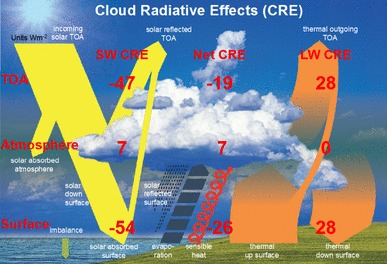
\includegraphics[scale = 7]{Chapter1_Intro/images/CRE_wild2019.jpg}
    \caption{Cloud radiative effect, CRE is the difference between the radiative components of the Clear sky radiative and the all sky. Cite this figure as fig 15 in Wild 2019. Skal få tak i denne figuren uten rød tall og redigere den selv.}
    \label{fig:cre}
\end{figure}

\begin{equation} \label{eq:cre_sw}
    CRE_{sw} = SW\uparrow_{clear-sky} - SW\uparrow_{all-sky}
\end{equation}

\begin{equation} \label{eq:cre_lw}
    CRE_{lw} = LW\uparrow_{clear-sky} - LW\uparrow_{all-sky}
\end{equation}

The physical properties causing the interaction with radiation is described below. Dense low level clouds reflect solar radiation. This is called the albedo effect. \textit{Albedo} being the ratio between reflected to incoming radiation. The higher number concentrations of droplets in a cloud the higher the total surface area of droplets. The more radiation gets reflected back into space. Clouds absorb longwave radiation and re-emits it. The absorbed radiation originates from the surface and is given by Stefan-Boltzmann forth-power law, see equation (\ref{eq:stefan-boltzmann}). The emissivity, $\epsilon$ depends on the (composition, compactness and surface roughness) of the medium. Water, snow and ice have different spectral emissivity. Huang et. al., 2018. Different parts of the globe are covered by different surfaces and Huang et al 2016 proved that assuming a constant surface emissivity effects effects the \acrshort{toa} polar energy budget. The greenhouse effect increases with the cloud altitude. Since high clouds have low temperatures and since the re-emitted radiation at a lower intensity than they absorbed. Researchers are still working on determine the emissivity of the different phases. Despite the uncertainties related to emissivity of the medium, the re-emitted radiation is of a lower intensity than what it absorb.

\begin{equation} \label{eq:stefan-boltzmann}
    F = \sigma \epsilon T ^4
\end{equation}

\section{Clouds in future climates} \label{sec:intro_cloud_future_climates}
\begin{figure}[h]
    \centering
    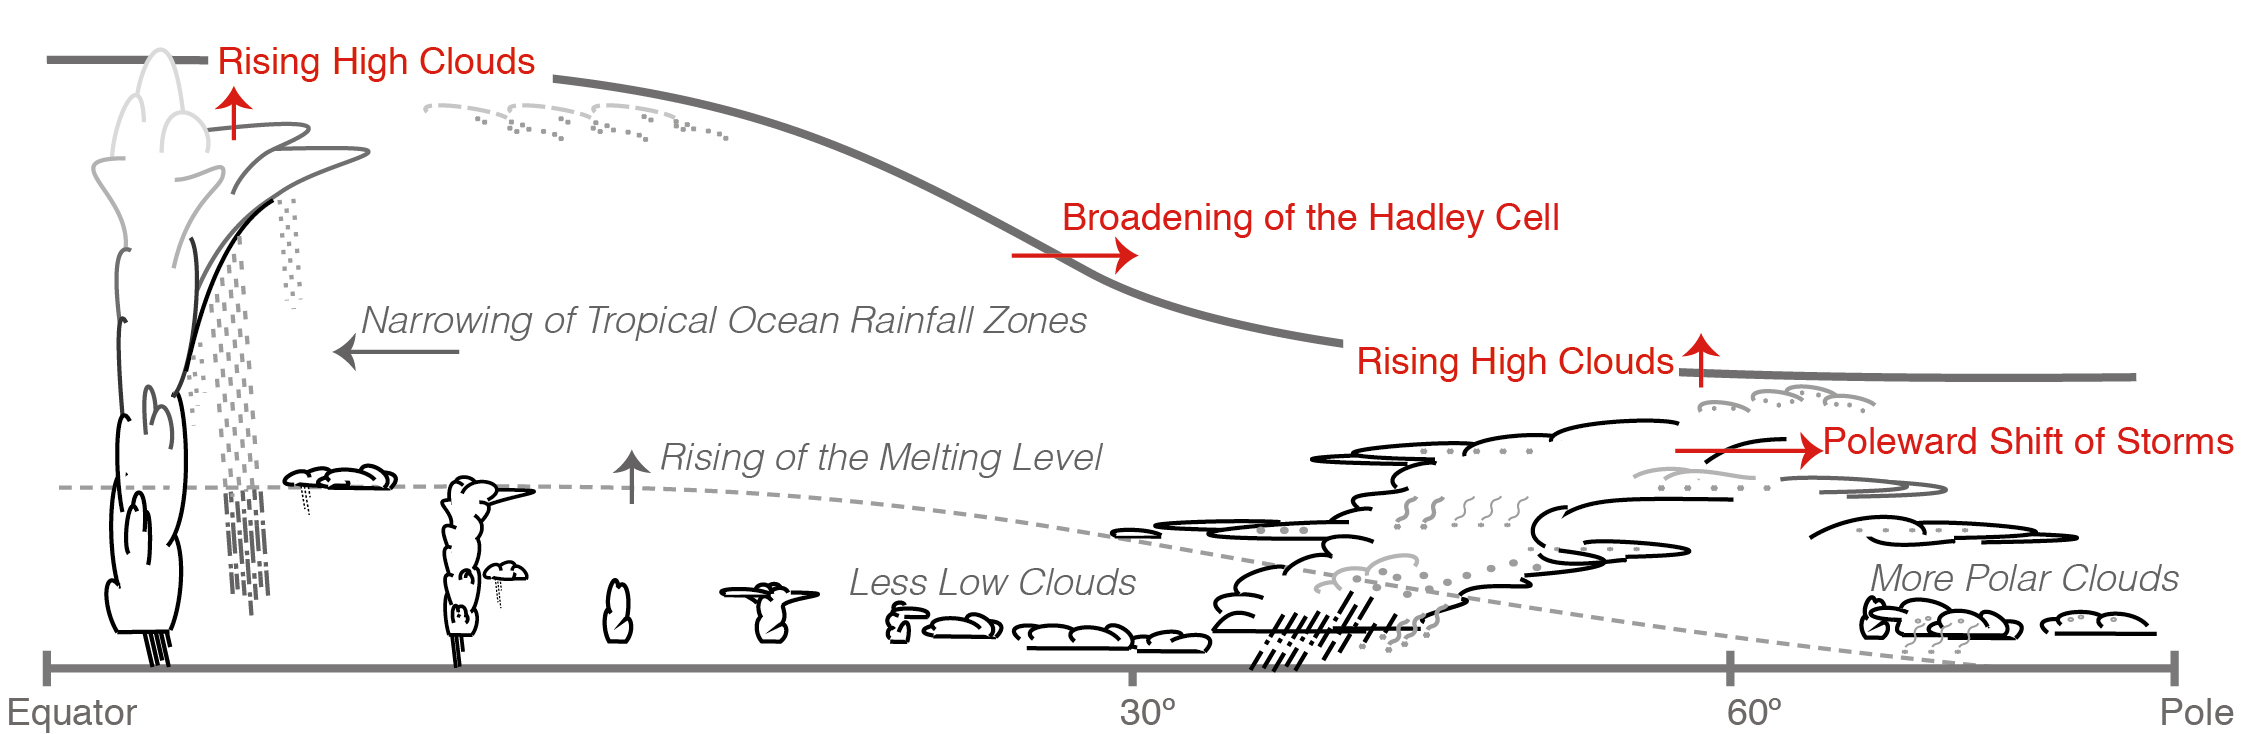
\includegraphics[scale = 0.8]{Chapter1_Intro/images/Fig7-11_ipcc.jpg}
    \caption{Cloud climatology in future climate. Developed based feedback's in climate models, the different adjustments have different sikkerhet. Cite the fifth assessment report IPCC report.}
    \label{fig:cloud_scheme}
\end{figure}

Excess of radiation gets trapped in the earth system, forcing the surface temperature to increase in order to close the radiative budget. The imbalance at the \acrfull{toa} is estimated by Wild et. al. 2019 to be $0.6W m^{-2}$. 
% Wild et. al. 2019  \textbf{siter} finds an imbalance of This heat gets trapped in the earth system, forcing the surface temperature to increase in order to close the radiative budget. 
%The imbalance in the radiative budget at \acrfull{toa} is the radiative forcing. 
Climate drivers include both natural and anthropogenic forcings. \textit{Forcings} can be everything from natural variability in the solar energy output, volcanic eruptions and greenhouse gas emissions. The climate science community works toward a common goal to determine the climate sensitivity as a function of forcing. Different socio-economic pathways result different temperature increase. The temperature increase induces climate changes. The \acrfull{ipcc} suggest the following shift in cloud schemes (see figure \ref{fig:cloud_scheme}). Figure \ref{fig:cloud_scheme} shows a summary of the most likely cloud feedback's. First, a broadening of the Hadley cell causes a poleward shift of storms. This dries up the subtropics %(\textit{Narrowing the rainfall zone above the tropics .. }) 
and moistens the higher latitudes. The clouds move further into the polar night, decreasing the albedo effect. The greenhouse effect of clouds still persist without sunlight leading to a net heating in the Arctic. Second, rising higher clouds causing a stronger greenhouse effect. Third, less low level clouds. This is assumed to be partly offset by a increase in the melting layer, leading to more opaque clouds. Rising of the meltlayer cause ice crystals to melt resulting in more opaque clouds. These opaque clouds a higher albedo and reflect more sunlight. 
\\ \\
Aerosols can alter the cloud micro-physics and in terms alter the radiative properties of the cloud. A polluted cloud receives additional \acrshort{ccn}. These share the available liquid. Reducing the size of droplets while increasing the number concentration. This increases the total surface area of the droplets resulting in more radiation reflected back to space. In fact, it takes smaller droplets longer to reach precipitation size, resulting in a enhanced lifetime. Precipitating clouds clean the air by removing particles. 
%\textbf{helt ny overgang til ML. evt. ikke tenk på det om avsnittet uansett flyttes.}
%Cloud micro-physical processes are not yet fully understood \textbf{kilde}. Together with the fact that clouds are formed a smaller scale then can be resolved in your average climate models. Parametrizations are used to include the contribution from the subgridscale processes to the mesoscale processes (weather phenomenons) in climate models and in weather predictions in general. Over the last years this has gained more attention since its acknowledged as the largest contributor to the uncertainty in climate models. I'll get back to this in section \ref{sec:update} .
